\documentclass[]{elsarticle}
%\documentclass[review]{elsarticle}

\usepackage{lineno,hyperref}
\modulolinenumbers[2]

\journal{Remote Sensing of Environment}

%%%%%%%%%%%%%%%%%%%%%%%
%% Elsevier bibliography styles
%%%%%%%%%%%%%%%%%%%%%%%
%% To change the style, put a % in front of the second line of the current style and
%% remove the % from the second line of the style you would like to use.
%%%%%%%%%%%%%%%%%%%%%%%

%% Numbered
%\bibliographystyle{model1-num-names}

%% Numbered without titles
%\bibliographystyle{model1a-num-names}

%% Harvard
%\bibliographystyle{model2-names.bst}\biboptions{authoryear}

%% Vancouver numbered
%\usepackage{numcompress}\bibliographystyle{model3-num-names}

%% Vancouver name/year
%\usepackage{numcompress}\bibliographystyle{model4-names}\biboptions{authoryear}

%% APA style
%\bibliographystyle{model5-names}\biboptions{authoryear}

%% AMA style
%\usepackage{numcompress}\bibliographystyle{model6-num-names}

%% `Elsevier LaTeX' style
\bibliographystyle{elsarticle-num}
%%%%%%%%%%%%%%%%%%%%%%%

\begin{document}

\begin{frontmatter}

\title{Understanding the drivers of diurnal and nocturnal urban land surface temperature}

%% or include affiliations in footnotes:
\author[1]{T.M. Logan\corref{mycorrespondingauthor}}
\cortext[mycorrespondingauthor]{Corresponding author}
\ead[url]{www.tomlogan.co.nz}
\ead{tomlogan@umich.edu}

\author[2]{B. Zaitchik}
\author[1]{S. Guikema}


\address[1]{Industrial and Operations Engineering, University of Michigan, Ann Arbor, MI}
\address[2]{Earth and Planetary Sciences, Johns Hopkins University, Baltimore, MD}

\begin{abstract}
Although heat waves and the urban heat island are nocturnal phenomenon, the drivers of land surface temperature during the night are poorly understood.
Given that heat waves are the deadliest natural hazard and are expected to increase in frequency and severity, determining mitigation strategies is important.
However, only recently has nocturnal imagery of cities become available by LandSat allowing nighttime land surface temperature to be analyzed.
Furthermore, it remains unclear from existing studies the independent effects of potential drivers, and their relative importance.
Here, we seek to answer the question: what are the effects and importance of drivers of land surface temperature during both day and night?
To do this, we analyze the urban land surface temperature in four cities across the United States.
We include factors related to vegetation, water, the built-environment, and topography and control them using nonlinear statistical methods which allow for their independent effects to be determined.
The results of diurnal and nocturnal analysis are compared to determine if previously reported relationships hold between cities and during both the day and night.
Understanding whether the factors related to high urban land surface temperatures are consistent across US cities is important for climate adaptation planning and during heat wave mitigation strategies.
\end{abstract}

\begin{keyword}

\end{keyword}

\end{frontmatter}

\linenumbers

\section{Introduction}
In a warming world, understanding the drivers of surface temperatures during both the day and night will aid in adapting cities to mitigate urban heat for the health and well being of communities.
Of all the natural events, heat waves are among the deadliest and are likely to become longer and more frequent with climatic changes.
Coupled with demographic shifts towards urban living, climate change puts significant impetus on reducing community exposure to heat waves.
An understudied aspect of urban land surface temperature are factors related to nocturnal surface temperature.
Nocturnal land surface temperature is important in heat wave mitigation given the urban heat island effect is most apparent during the night and the minimum nocturnal temperature is linked with heat stress and mortality.



\section{Data and Methods}


\section{Results and Discussion}

\subsection{Variables related to Land Surface Temperature}


\begin{figure}[h]
\begin{center}
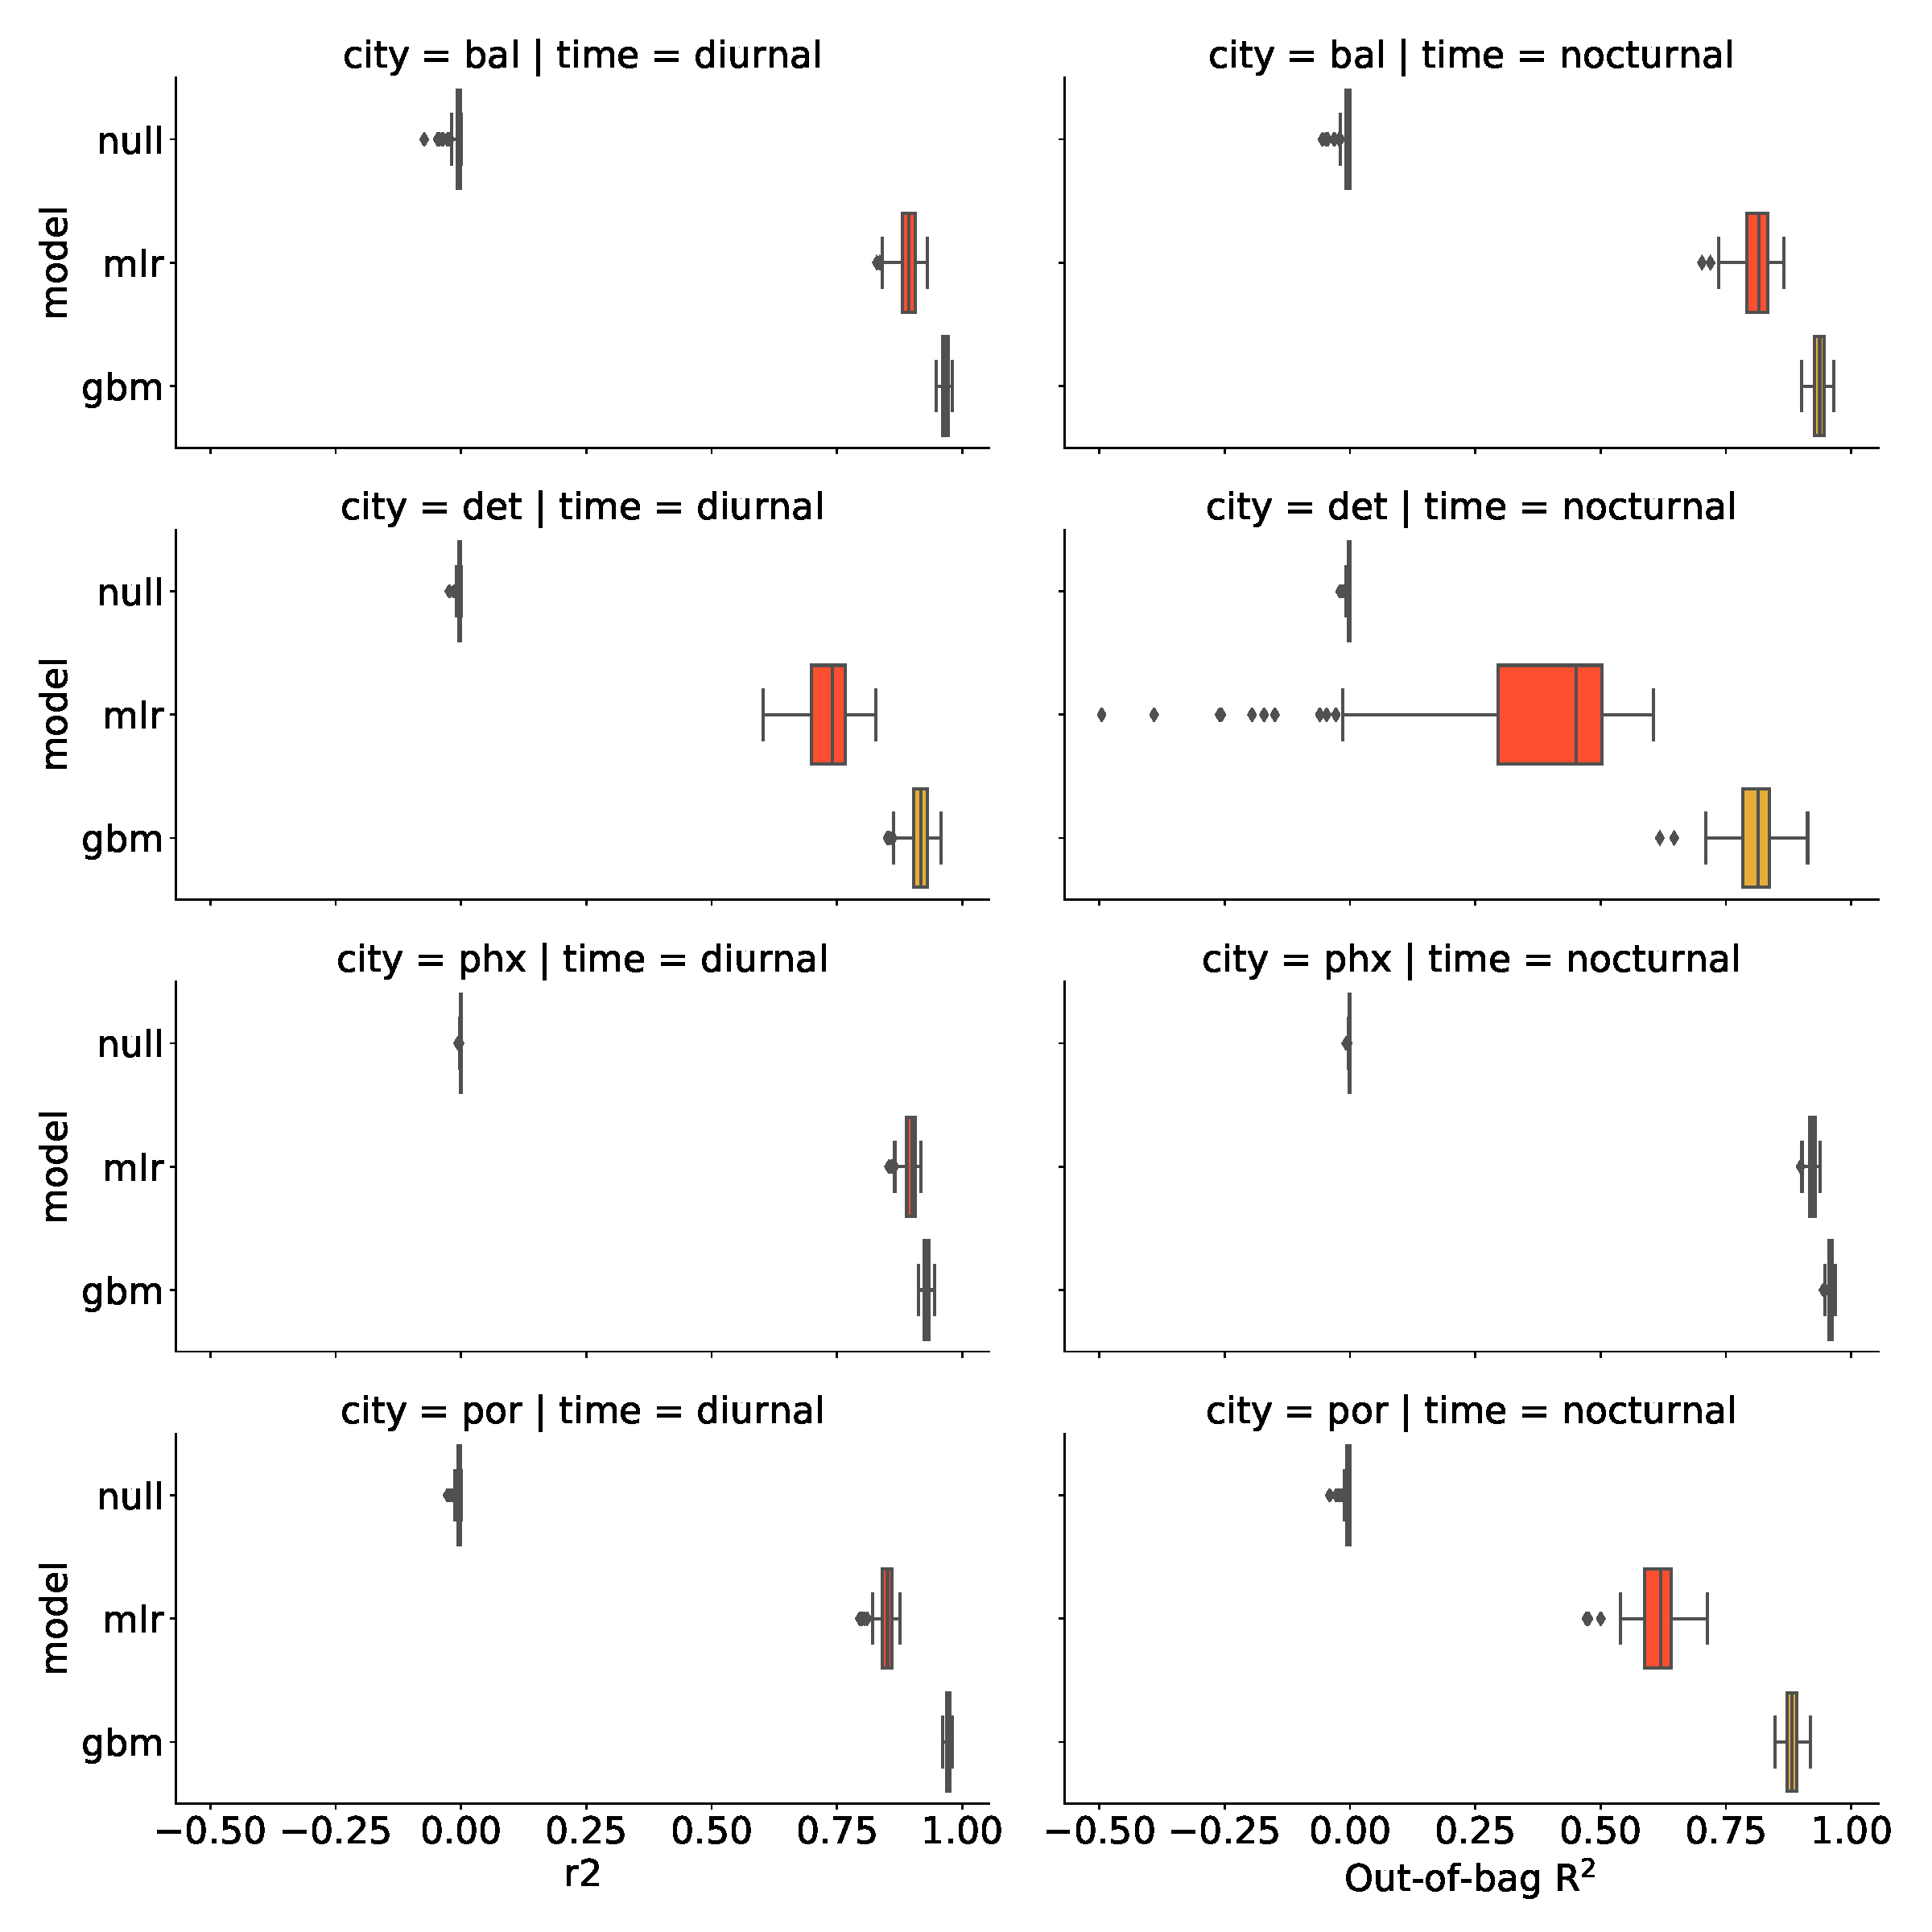
\includegraphics[width=\textwidth]{fig/report/holdout_results_r2.pdf}
\caption{The out-of-bag R$^2$ of the models when fitted on each city and used to predict a random sample from the same city. Out-of-bag R$^2$ can vary between $(-\infty, 1)$, where better models have a value near 1. This shows that the gradient boosted regression forest (gbm) consistently outperforms the multiple linear regression and null models.}
\label{fig:intracity}
\end{center}
\end{figure}


\subsection{Predicting Land Surface Temperature Between Cities}

See figure \ref{fig:intercity}.

\begin{figure}[h]
\begin{center}
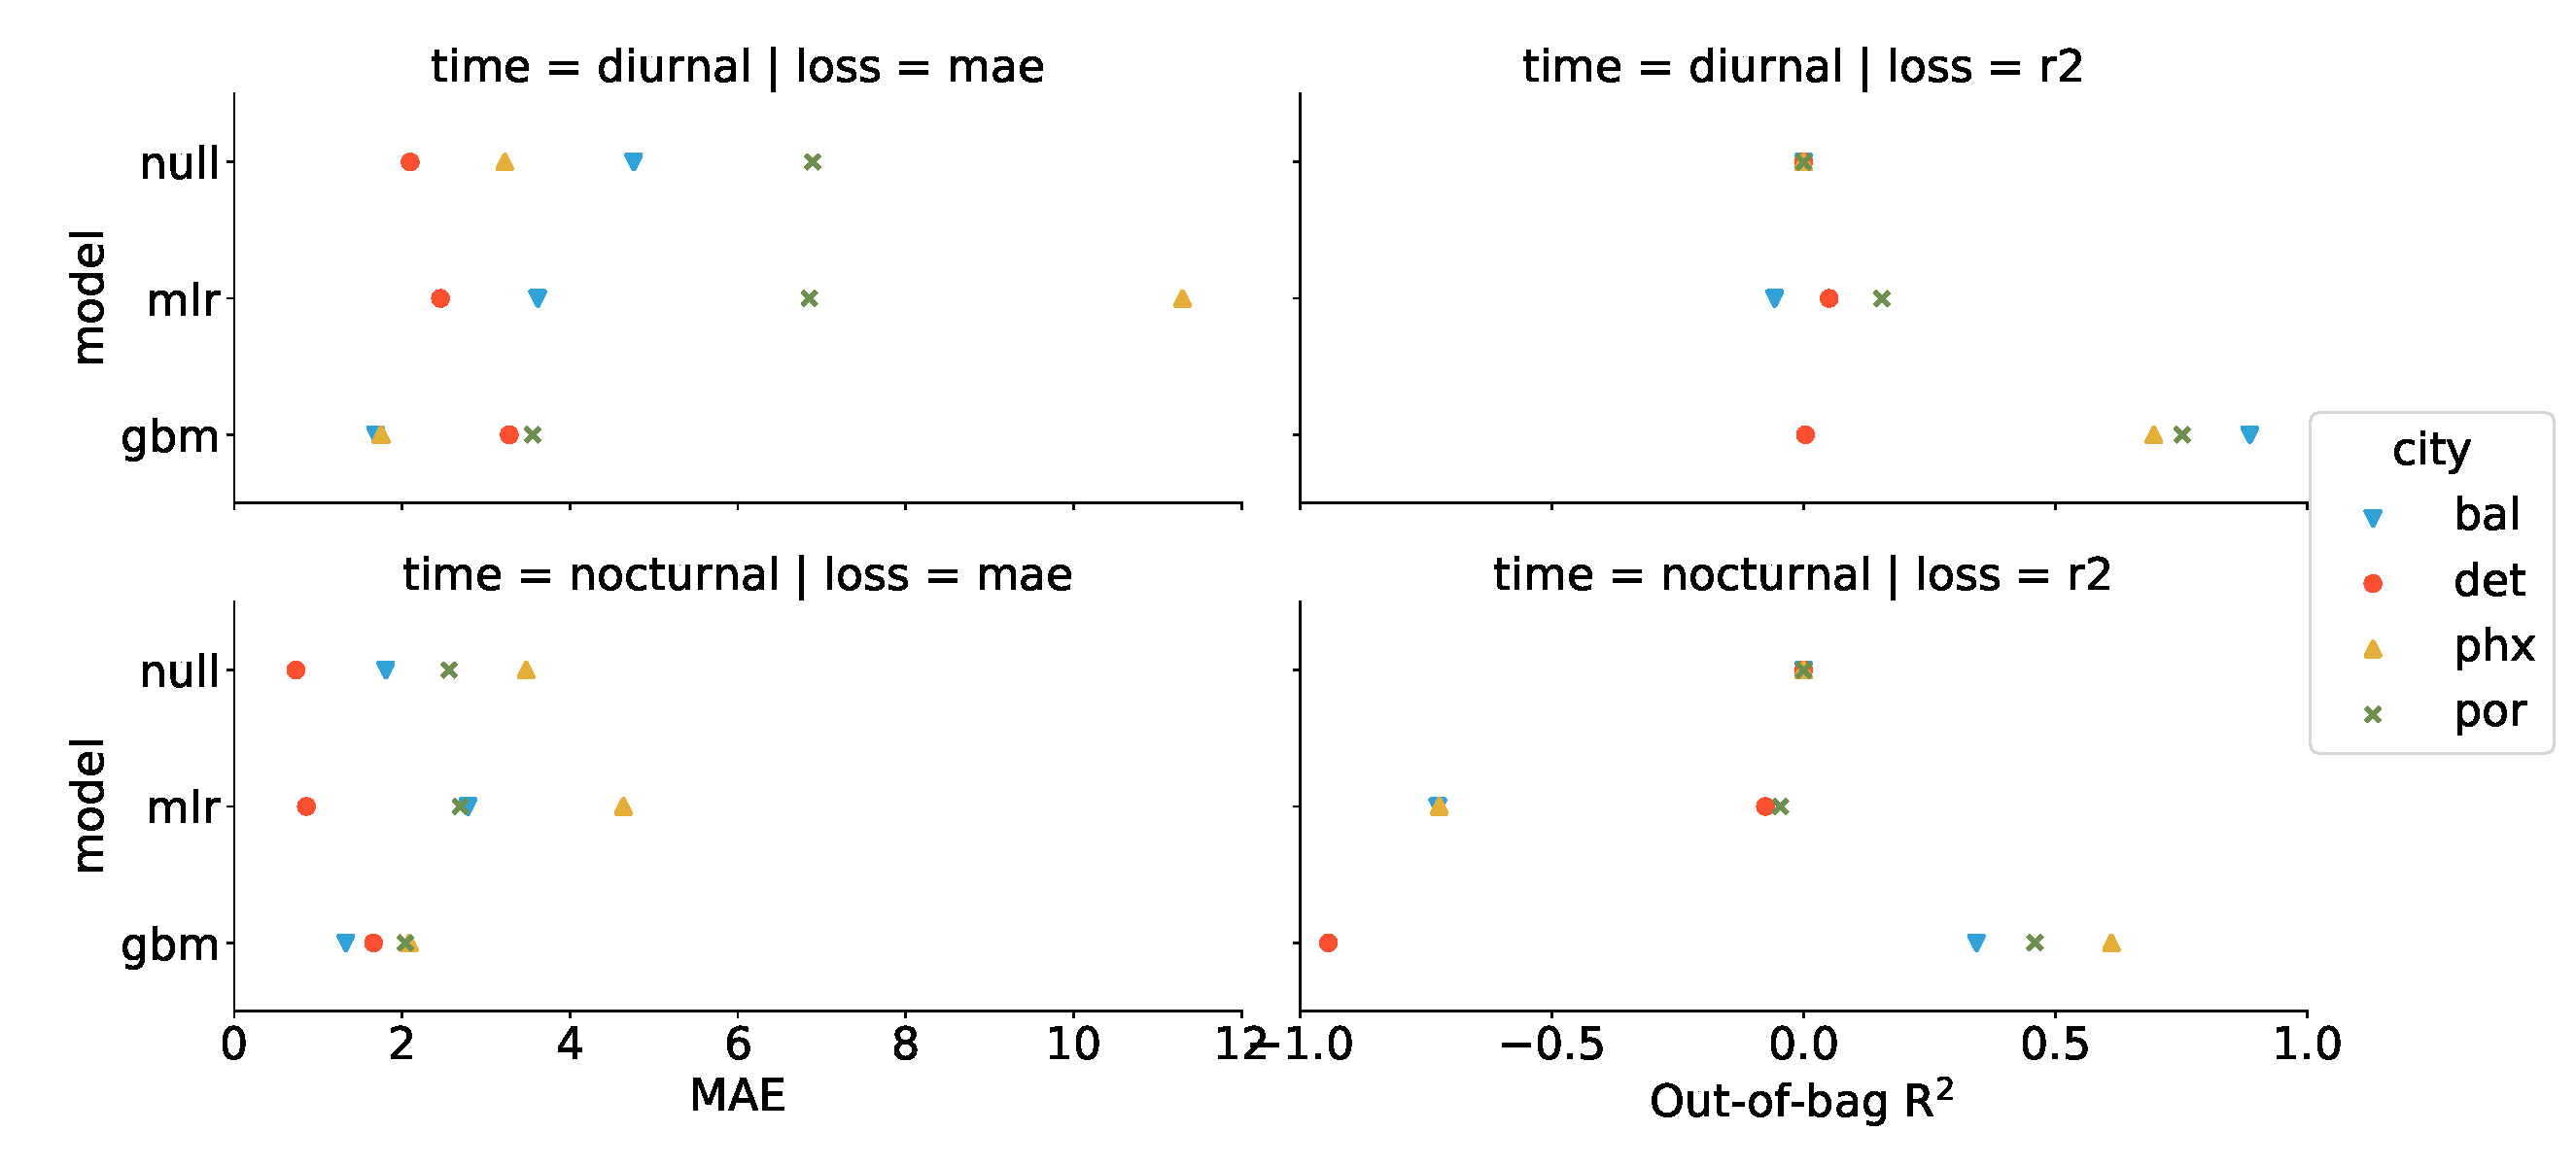
\includegraphics[width=\textwidth]{fig/report/cities_holdout.pdf}
\caption{The out-of-bag (OOB) R$^2$ and mean absolute error (MAE) of the models when fitted on three of the four cities and then used to predict the remaining city. OOB R$^2$ can vary between $(-\infty, 1)$, where better models have a value near 1. Good models have MAE near 0. The gradient boosted regression forest generally outperforms the other models, except when predicting Detroit. Note that the R$^2$ axis is truncated at -1, although the multiple linear regression for diurnal land surface temperature tested on Phoenix has an OOB R$^2$ of -9.  This shows that the gradient boosted regression forest (gbm) consistently outperforms the multiple linear regression and null models.}
\label{fig:intercity}
\end{center}
\end{figure}


\section{Drivers of LST}
See figure \ref{fig:importance} and \ref{fig:pdp}.

Regarding Fig \ref{fig:pdp}, I think I will remove the ``all" line, because in cases such as $alb_mean_min_sl$ (which is the minimum albedo in the surrounding cells (sl = spatial lag)) the values between the cities don't overlap so I think it becomes a proxy for other differences between the city when regressed together.

\begin{figure}[h]
\begin{center}
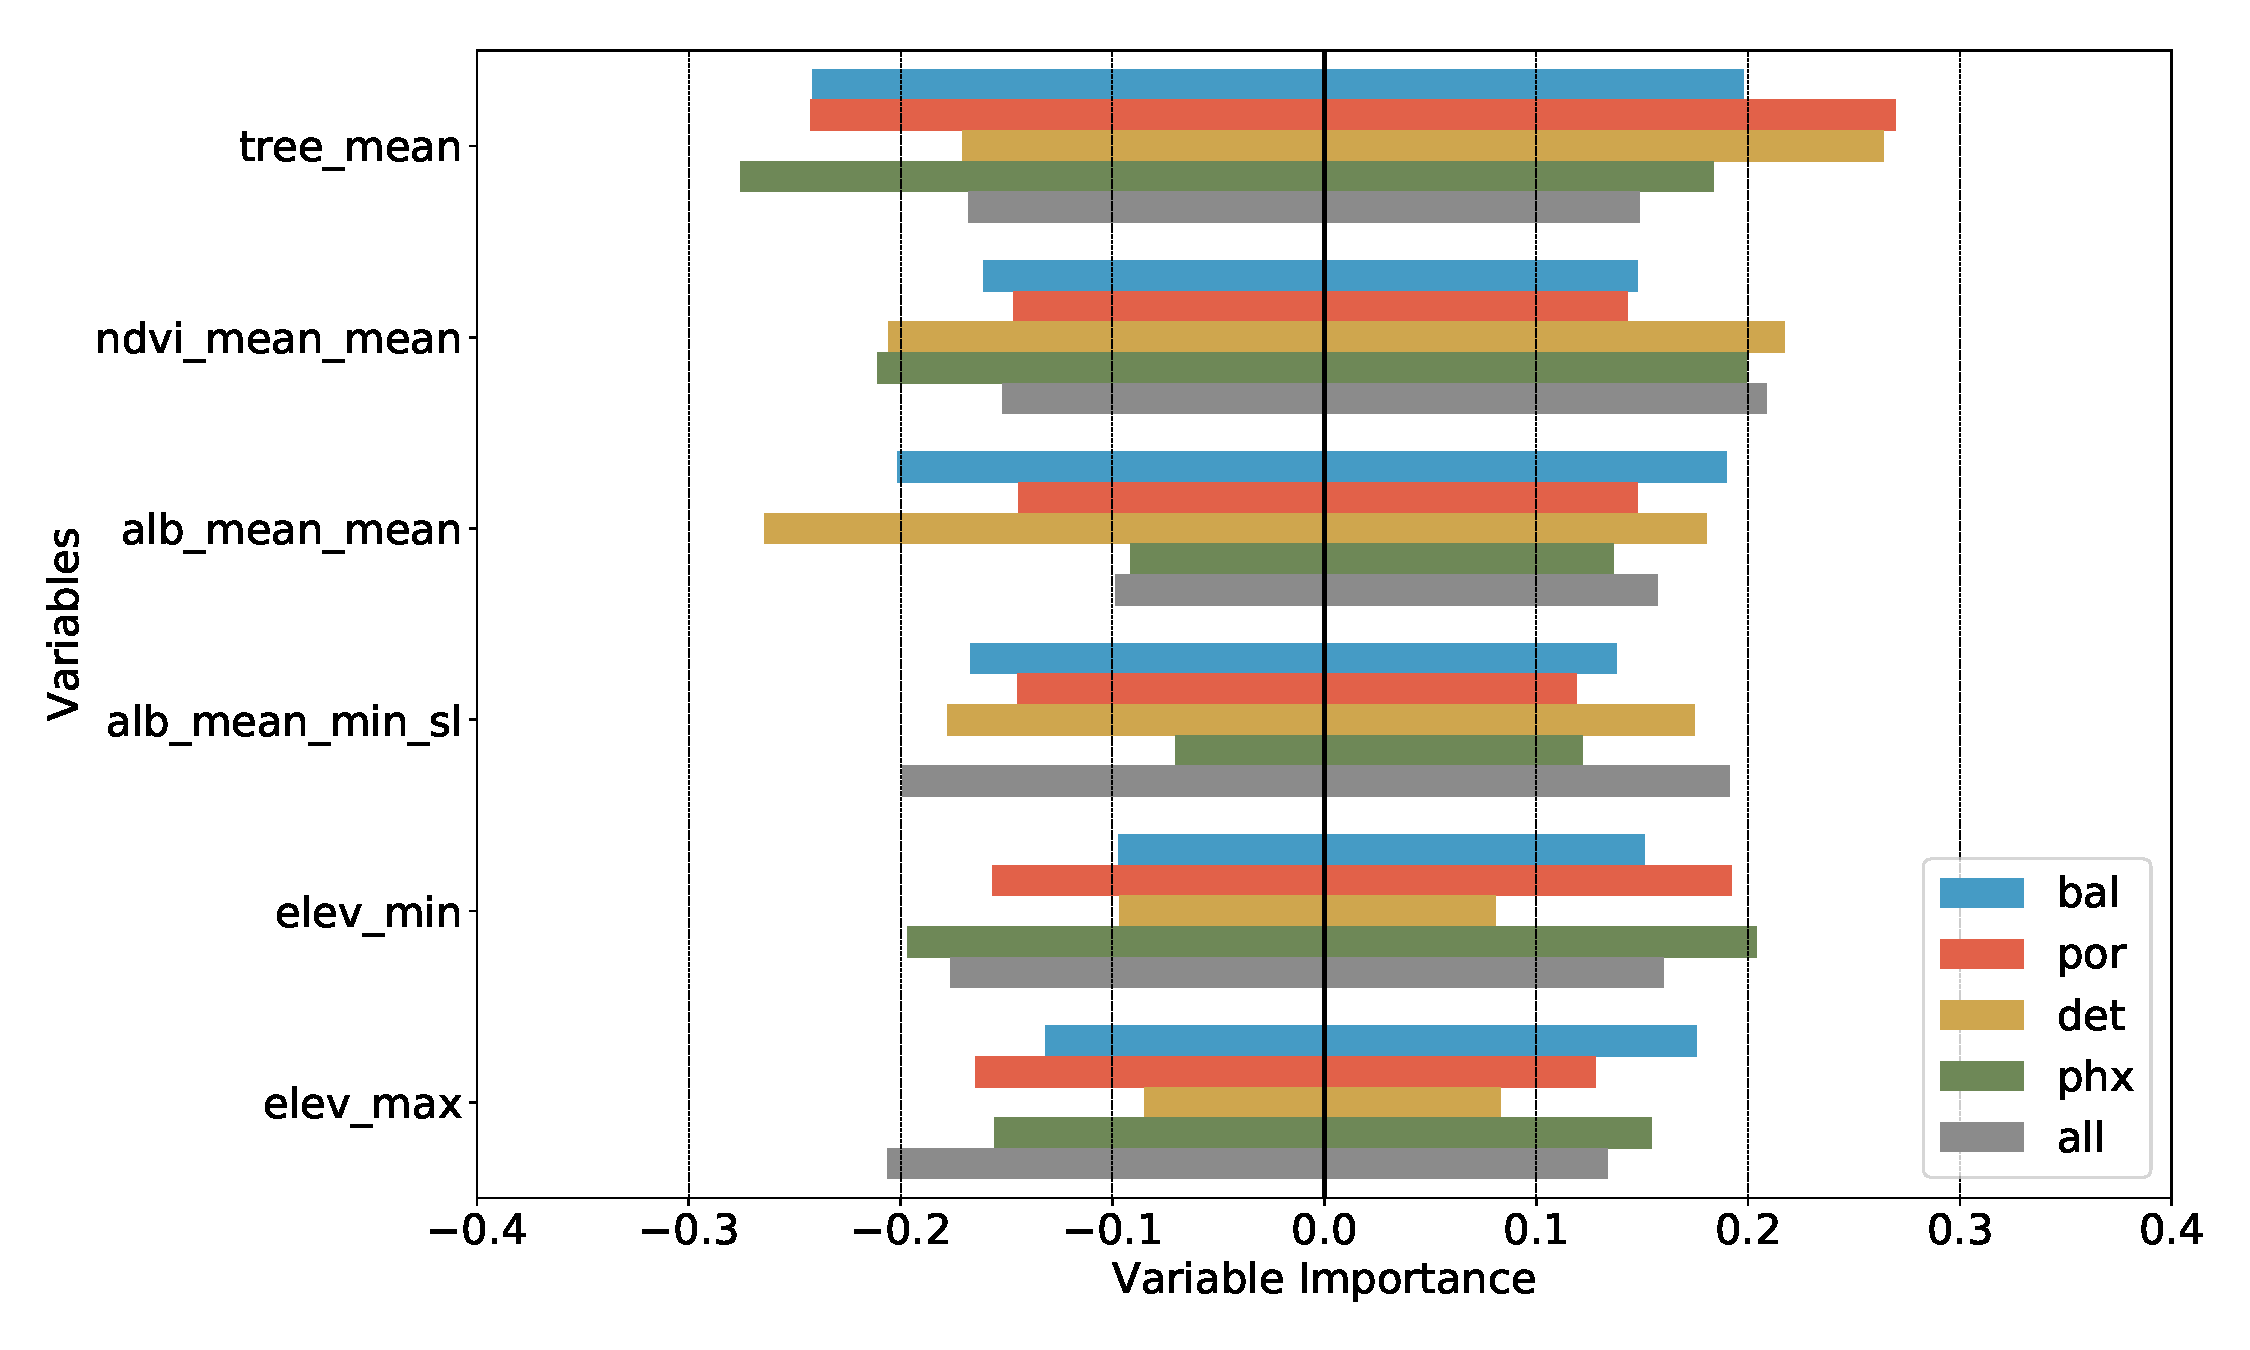
\includegraphics[width=\textwidth]{fig/report/variable_importance_selected.pdf}
\caption{The variable importance for the regression during the night (to the left) and the day (to the right). Variable importance indicates the amount that each variable improves the performance of the regression.
In this case there is generally little difference between the importance of day and night variables.}
\label{fig:importance}
\end{center}
\end{figure}

\begin{figure}[h]
\begin{center}
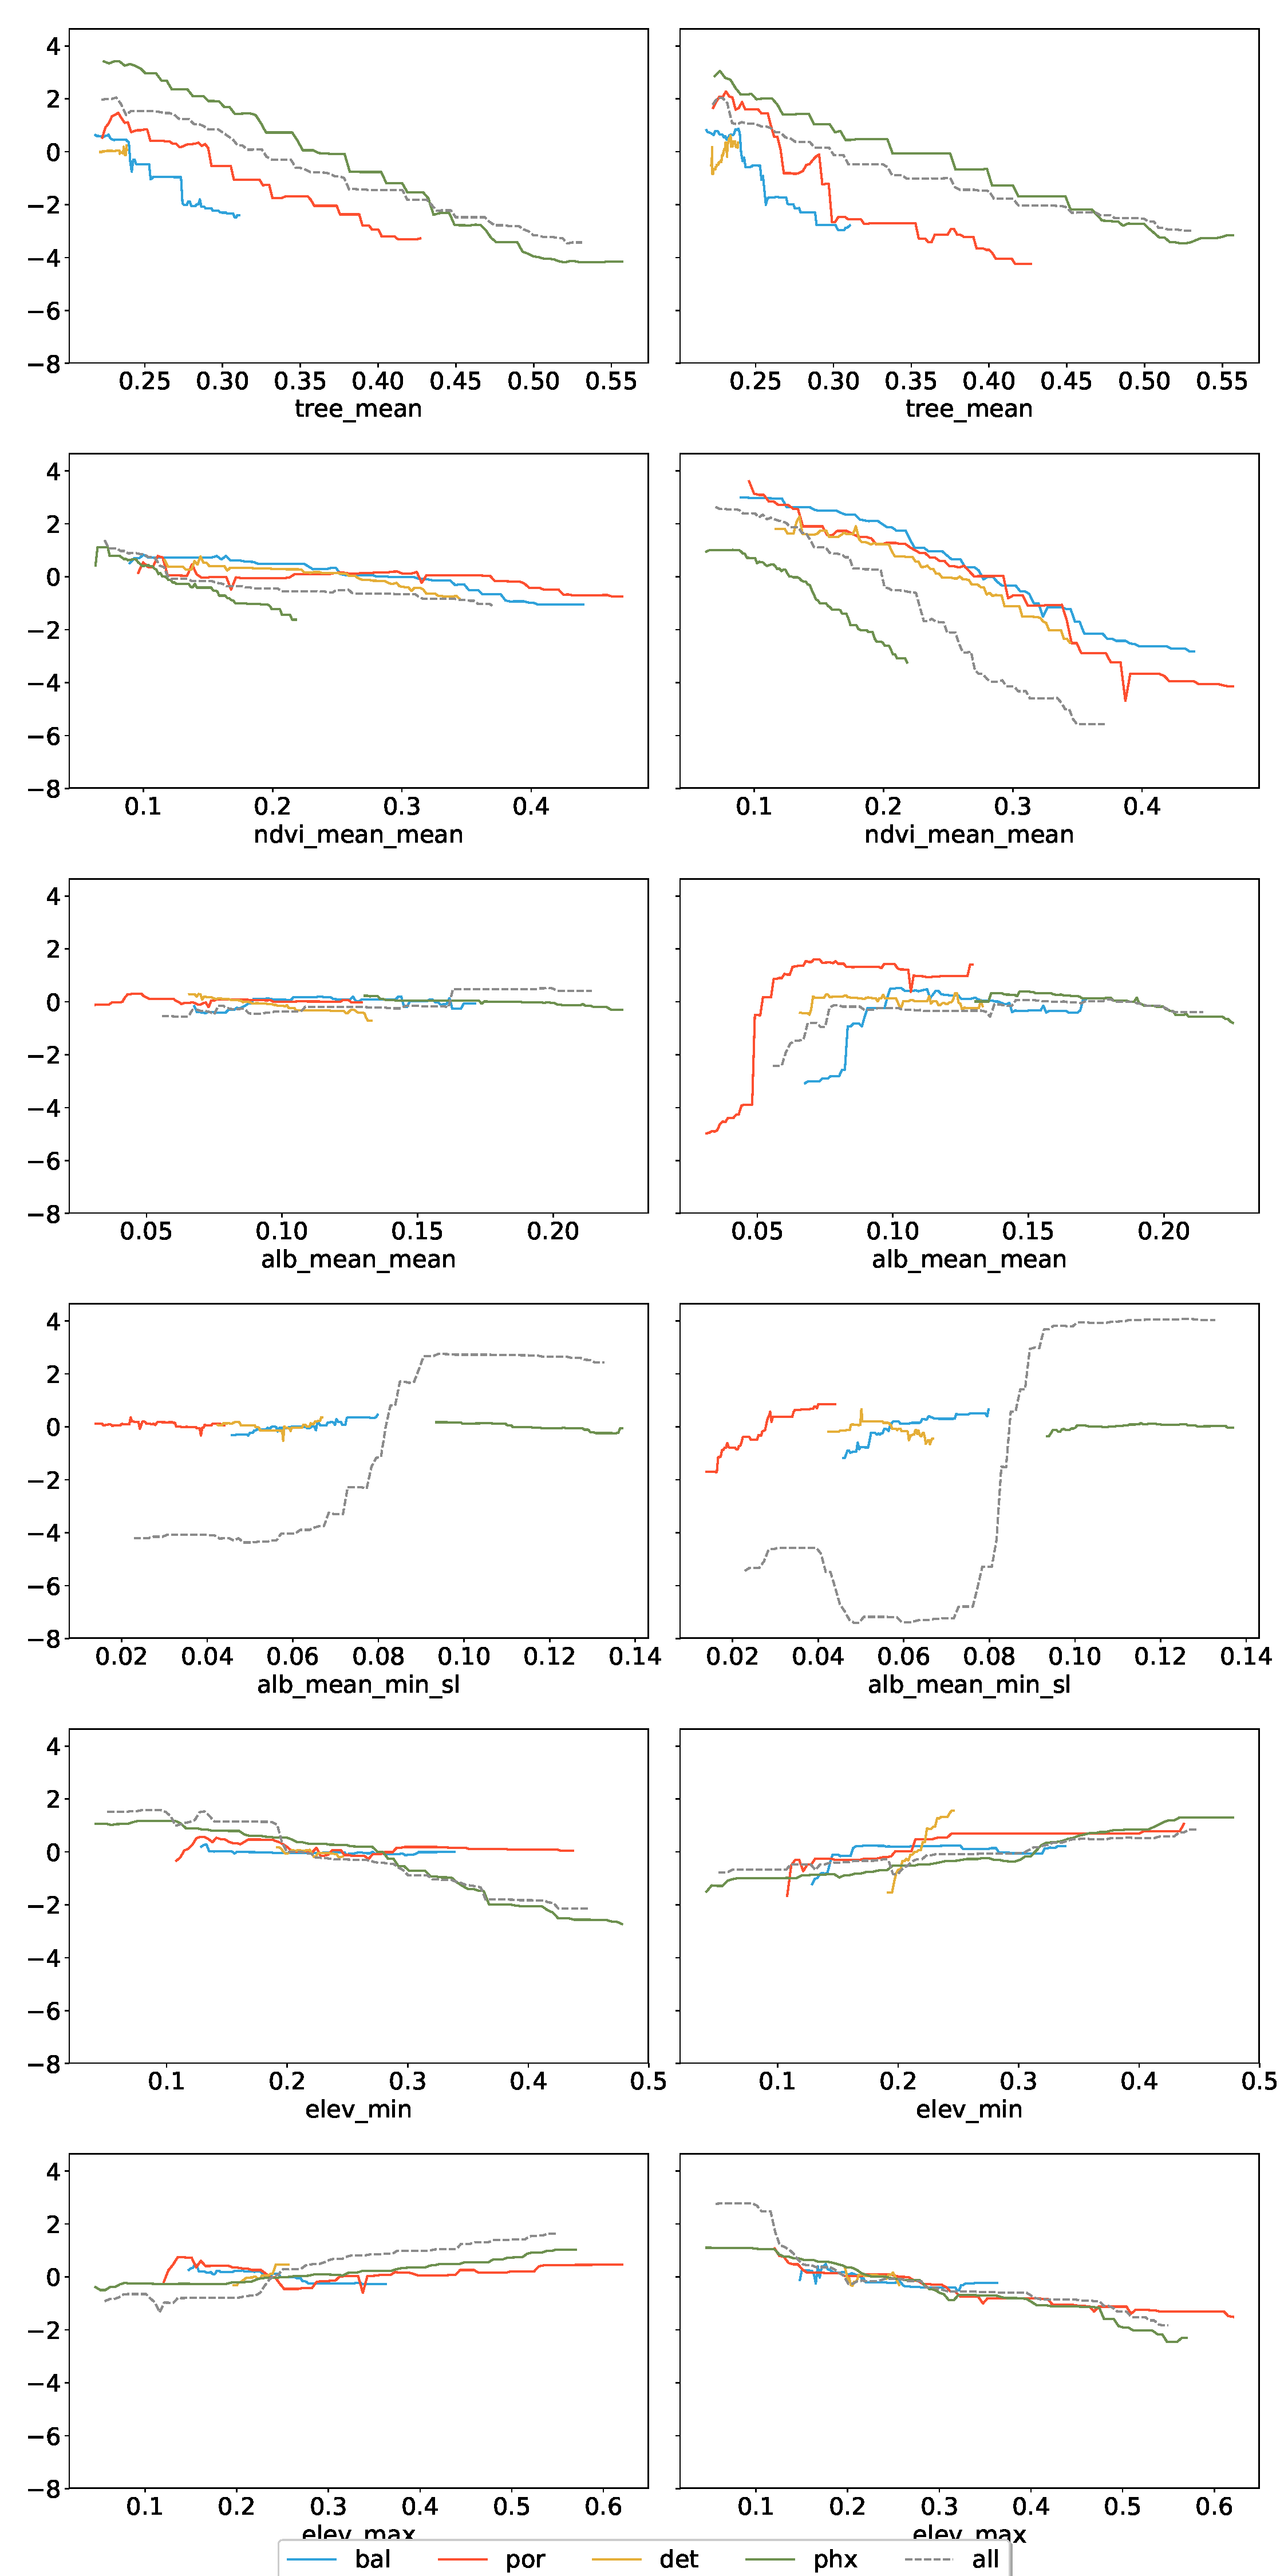
\includegraphics[height=\textheight]{fig/report/partial_dependence.pdf}
\caption{Partial dependence plots show how the land surface temperature ($^oC$, y axis) changes with each variable as the other variables are held at their average value. The left hand side shows the effect each variable has on LST during the night, while the right hand side shows the effect during the day. This shows that trees coverage in the cell has the greatest influence on the temperature, and the greenness (NDVI) of that coverage matters during the day.}
\label{fig:pdp}
\end{center}
\end{figure}



% \section{Conclusion}

% There are various bibliography styles available. You can select the style of your choice in the preamble of this document. These styles are Elsevier styles based on standard styles like Harvard and Vancouver. Please use Bib\TeX\ to generate your bibliography and include DOIs whenever available.

% Here are two sample references: \cite{Feynman1963118,Dirac1953888}.

% % \section*{References}

% \bibliography{mybibfile}

\appendix
\section{2013 Land Surface Temperature Image}


\section{Additional model results}
\begin{figure}[h]
\begin{center}
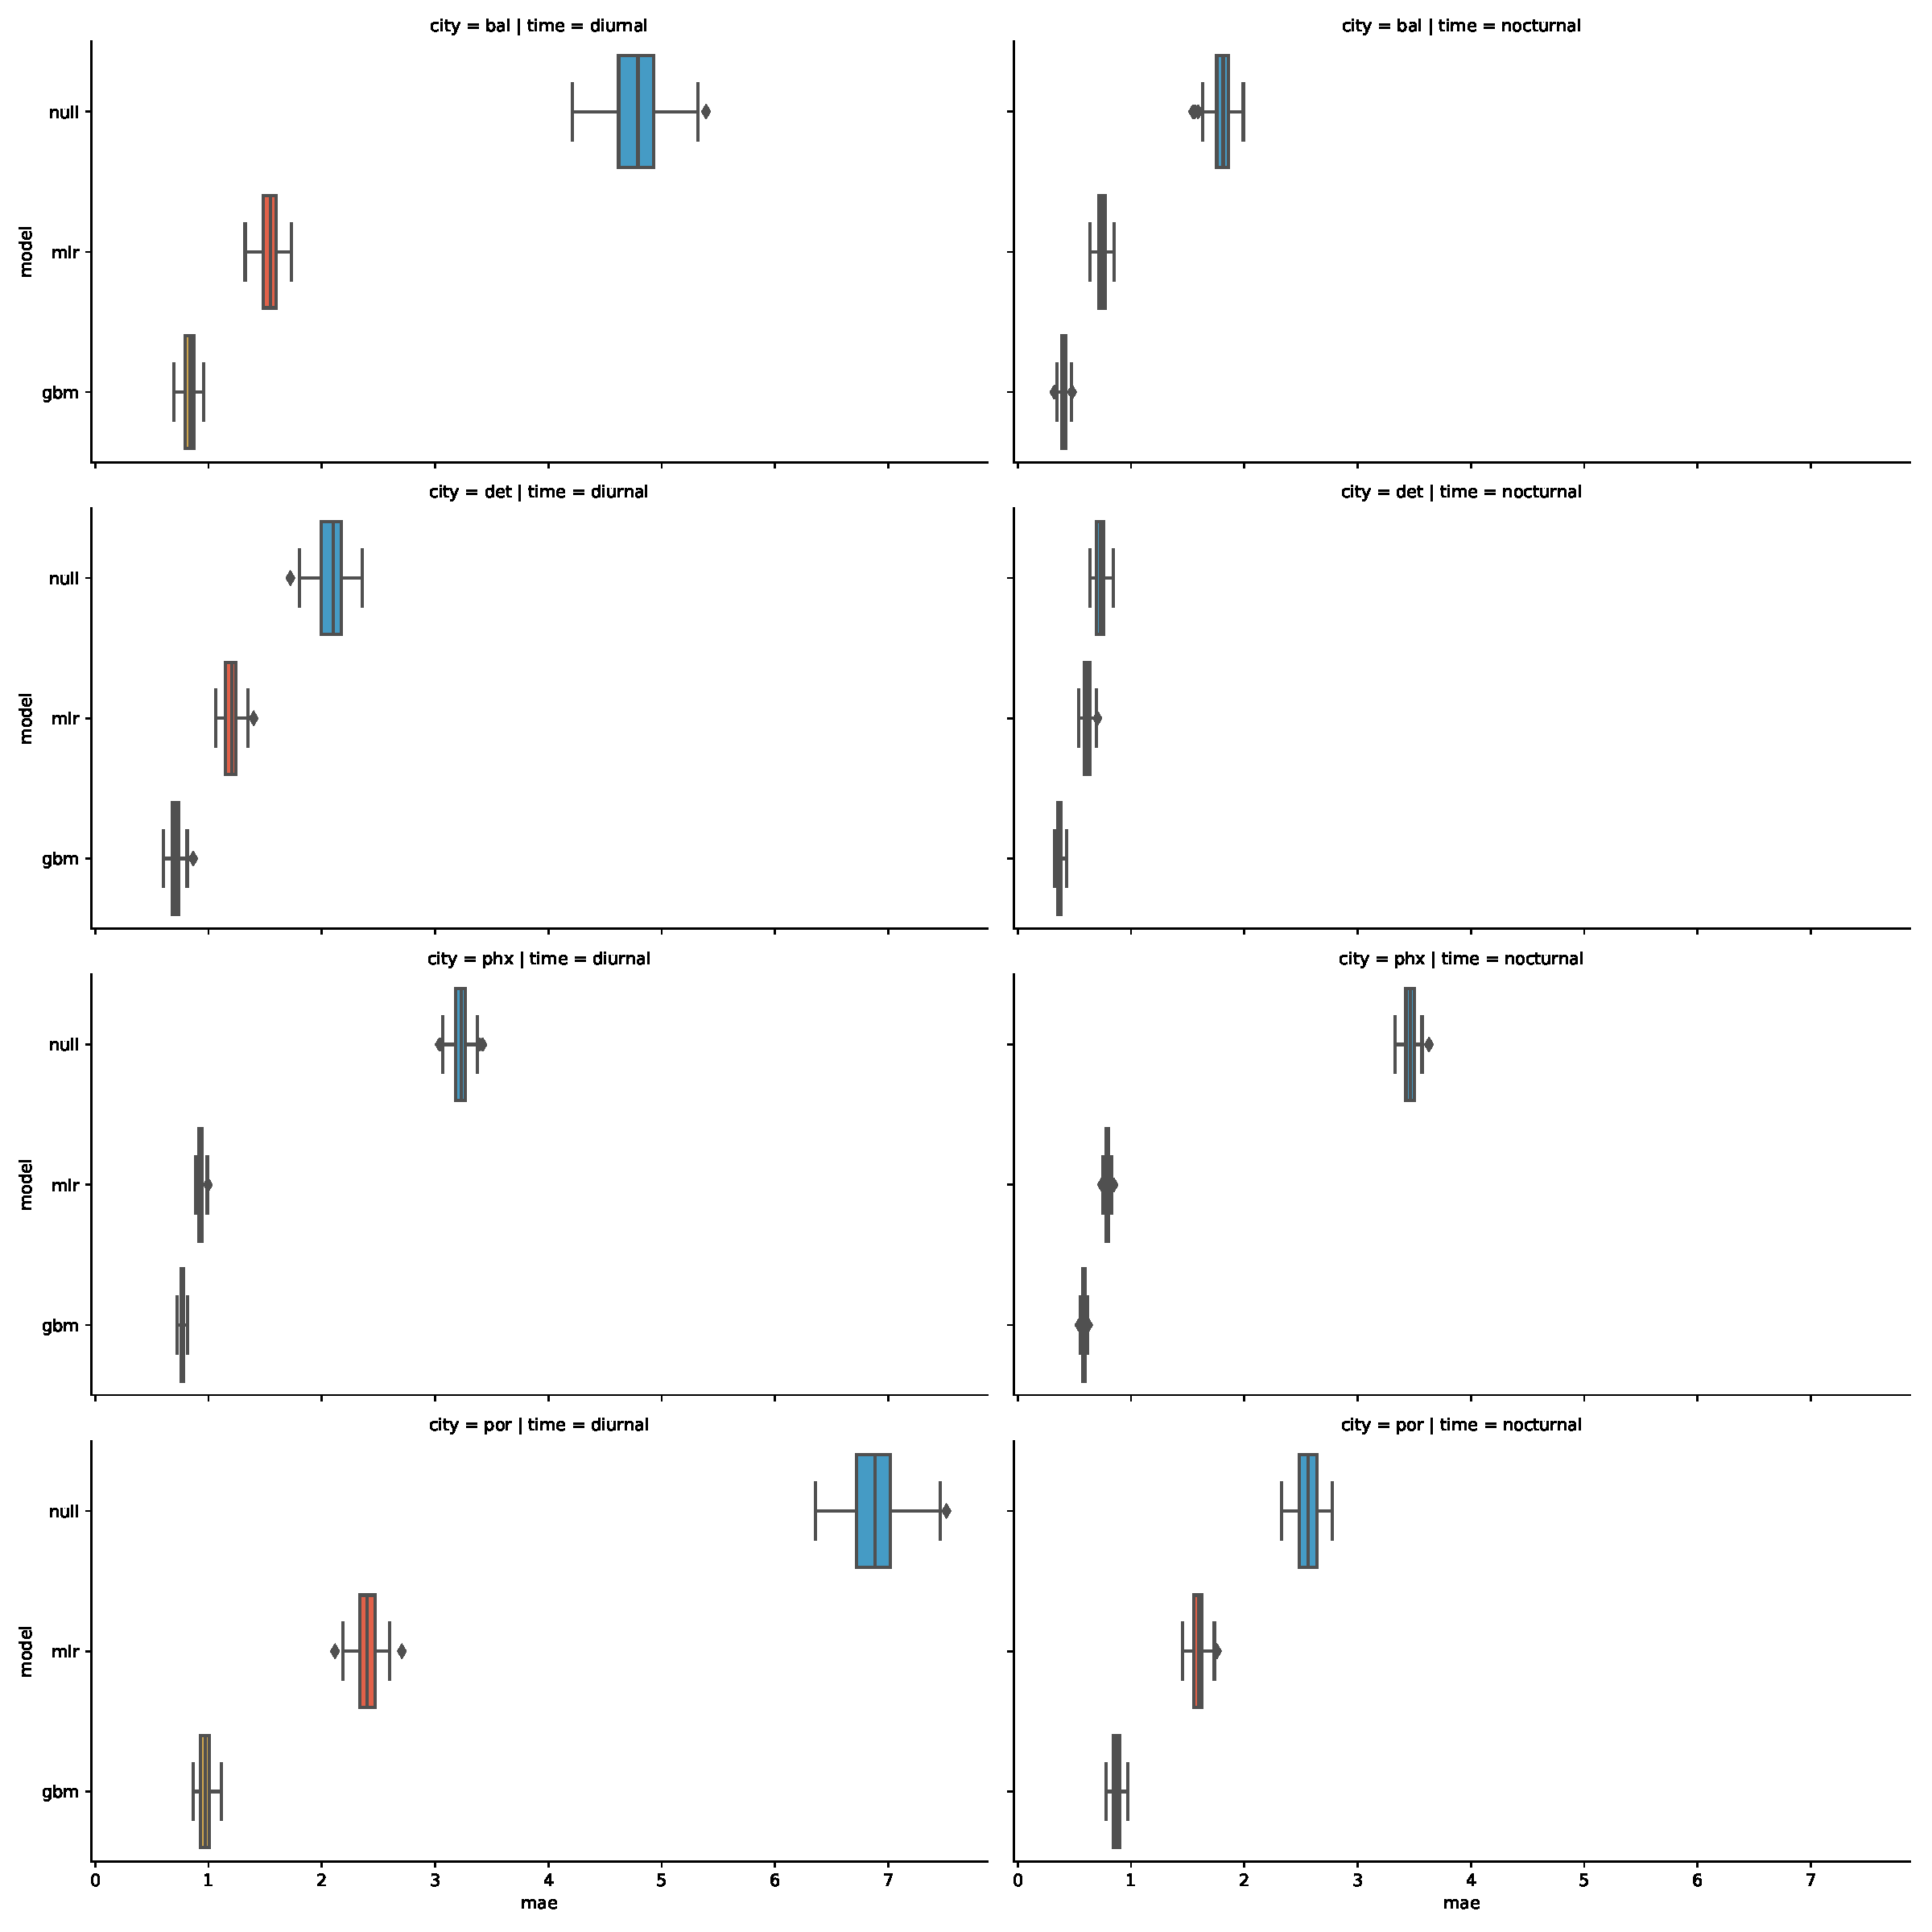
\includegraphics[width=\textwidth]{fig/report/holdout_results_mae.pdf}
\caption{The Mean Absolute Error (MAE) in $^oC$ of the models when fitted on each city and used to predict a random sample from the same city. Better models have lower MAE. This shows that the gradient boosted regression forest (gbm) consistently outperforms the multiple linear regression and null models. }
\label{fig:cityholdout_errors}
\end{center}
\end{figure}




\end{document}
